\documentclass[11pt,english,compress]{beamer}

\usepackage[utf8]{inputenc}
\usepackage{verbatim}
\usepackage{eurosym}
\usepackage{stmaryrd}

\usepackage[compatibility=false]{caption}
\usepackage{subcaption}
\usepackage{pgfplots}

\useoutertheme[subsection=false]{smoothbars}
\useinnertheme[shadow=true]{rounded}

\usecolortheme{orchid}
\usecolortheme{whale}

\setcounter{tocdepth}{2}
\setcounter{secnumdepth}{0}

\setbeamertemplate{footline}[frame number]

\title{The Linux graphics stack, Optimus and the Nouveau driver}
\subtitle{Cooperative rendering across GPUs on Linux}
\author{Martin Peres}
\institute{Nouveau developer\\PhD student at LaBRI\\X.Org Foundation board member}

\AtBeginSection[]{
  \begin{frame}{Summary}
  \small \tableofcontents[currentsection, hideothersubsections]
  \end{frame} 
}

\begin{document}

\setbeamertemplate{navigation symbols}{}
\setbeamertemplate{footline}[frame number]

\begin{frame}[plain,noframenumbering]
	\titlepage
\end{frame}

\section{Introduction to the Linux graphics stack}
\subsection{General overview}
\begin{frame}
	\frametitle{General overview of the Linux Graphics stack}

	\begin{block}{The graphics stack before 2005}
		\begin{itemize}
			\item The X-Server provided everything:
			\begin{itemize}
				\item Modesetting (CRTC \& plane management);
				\item 2D/3D acceleration;
				\item Video rendering acceleration;
				\item Input management.
			\end{itemize}
			\item The X-Server talked to the GPU directly, as root.
		\end{itemize}
	\end{block}

	\begin{block}{The current graphics stack}
		\begin{itemize}
			\item The X-Server got split into more than 200 components:
			\begin{itemize}
				\item Privileged operations moved to the kernel;
				\item 2D drivers got put into different shared objects;
				\item 3D acceleration got put in mesa;
				\item The list is too long ;)
			\end{itemize}
		\end{itemize}
	\end{block}
\end{frame}

\begin{frame}
	\begin{figure}[h]
		\centering
		\includegraphics[width=1.02\linewidth]{imgs/Linux_Graphics_Stack_2013.pdf}
		\caption{General overview of the Linux graphics stack}
	\end{figure}
\end{frame}

\subsection{Kernel space}

\begin{frame}
	\frametitle{The kernel space}

	\begin{block}{Direct Rendering Manager (DRM) : The common code}
		\begin{itemize}
			\item This common code provides:
			\begin{itemize}
				\item Kernel ModeSetting (KMS): CRTC \& plane management;
				\item Video memory management via GEM (with a TTM backend?);
				\item Nodes with different capabilities (master or render nodes).
			\end{itemize}
		\end{itemize}
	\end{block}

	\begin{block}{DRM open source drivers}
		\begin{itemize}
			\item i810/i915: Intel;
			\item nouveau: NVIDIA;
			\item radeon: AMD/ATI;
			\item vmwgfx: VMware;
			\item many SoC GPUs (armada, exynos, msm, omap, tegra, ...).
		\end{itemize}
	\end{block}
\end{frame}

\subsection{User space}

\begin{frame}
	\frametitle{Architecture of the X-Server}

	\begin{figure}[h]
		\centering
		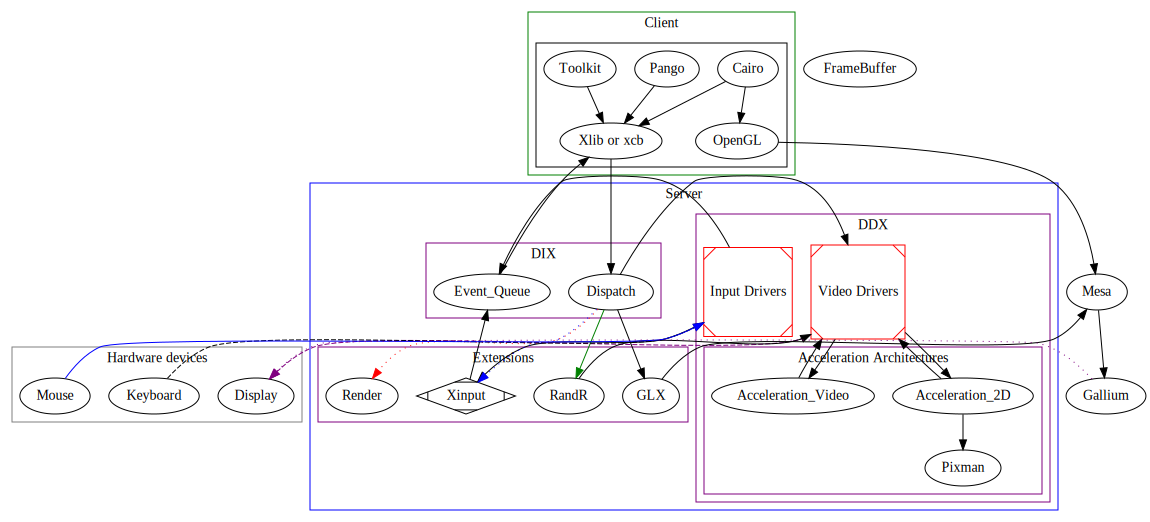
\includegraphics[width=1\linewidth]{imgs/xorg.pdf}
		\caption{General overview of the X-Server's internal architecture}
	\end{figure}
\end{frame}

\begin{frame}
	\frametitle{Architecture of Mesa}

	\begin{figure}[h]
		\centering
		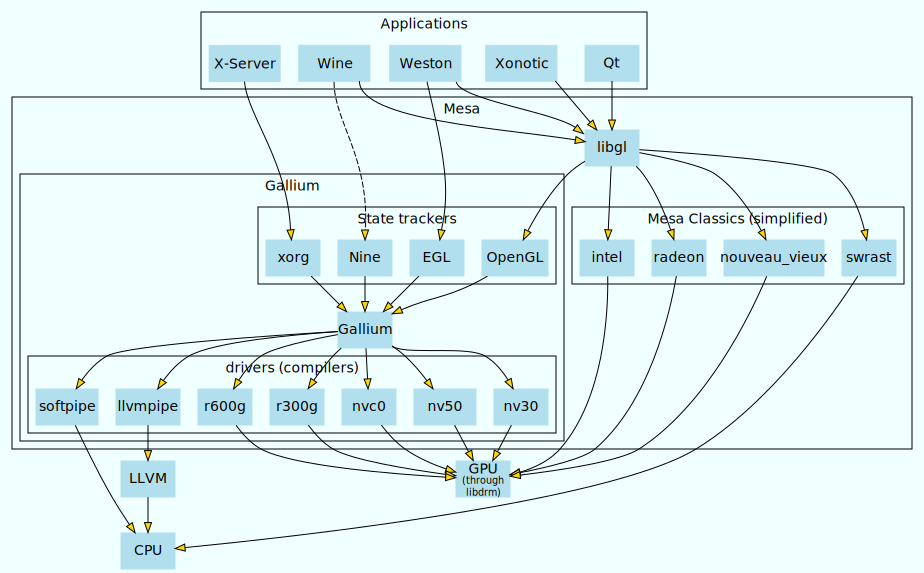
\includegraphics[width=1\linewidth]{imgs/mesa.pdf}
		\caption{General overview of Mesa's internal architecture}
	\end{figure}
\end{frame}

\section{Optimus}
\subsection{Introduction}
\begin{frame}
	\frametitle{Great performance, great battery-life}

	\begin{block}{Optimus}
		\begin{itemize}
			\item Laptops can be equipped with two GPUs;
			\item The Intel IGP is great for battery-life;
			\item NVIDIA's discrete GPU (dGPU) is great for performance;
			\item Dynamic switch between the 2: get the best of both worlds!
		\end{itemize}
	\end{block}

	\begin{block}{Challenges}
		\begin{itemize}
			\item When/How the dGPU should be turned on/off?
			\item Who drives the outputs?
			\item How to copy buffers from a driver to another?
			\item How should we handle the HDMI ``sound card''?
		\end{itemize}
	\end{block}
\end{frame}

\subsection{Turning the dGPU on/off}
\begin{frame}
	\frametitle{Turning the dGPU on/off}

	\begin{block}{How}
		\begin{itemize}
			\item Optimus laptops have ACPI functions to do that;
			\item Two ways of calling them:
			\begin{itemize}
				\item bbswitch: Old kernel module for manual management;
				\item vgaswitcheroo: Manual or automatic state management.
			\end{itemize}
		\end{itemize}
	\end{block}

	\begin{block}{When: The case of vgaswitcheroo}
		\begin{itemize}
			% \item can't remember what I wanted to write here!
			\item Turn off the dGPU when it has been idle for 5 seconds;
			\item Idle?: 
			\begin{itemize}
				\item no graphics context allocated;
				\item no output is being used;
				\item no sound interface used (not done);
				\item no call to the drm driver has been made;
			\end{itemize}
		\end{itemize}
	\end{block}
\end{frame}

\subsection{Driving the right outputs}
\begin{frame}
	\frametitle{Handling the outputs : Hardware multiplexer}

	\begin{figure}[h]
		\centering
		\includegraphics[height=7cm]{imgs/optimus_hw_mux.png}
		\caption{Switchable graphics}
	\end{figure}
\end{frame}

\begin{frame}
	\frametitle{Handling the outputs : Software multiplexer}

	\begin{figure}[h]
		\centering
		\includegraphics[height=7cm]{imgs/optimus_sw_mux.png}
		\caption{The ``real'' Optimus architecture}
	\end{figure}
\end{frame}

\begin{frame}
	\frametitle{Switching from one GPU to another : How windows does it}

	\begin{figure}[h]
		\centering
		\includegraphics[width=1\linewidth]{imgs/optimus_arch.png}
		\caption{The global hardware/software infrastructure}
	\end{figure}
\end{frame}

\subsection{How to share buffers across drivers?}

\begin{frame}
	\frametitle{Sharing buffers across drivers}

	\begin{block}{Challenges}
		
		\begin{itemize}
			% \item can't remember what I wanted to write here!
			\item The memory representation for buffers is different from hardware to hardware:
			\begin{itemize}
				\item pitch: number of pixels per row;
				\item tiling: technique that increases the spatial locality.
			\end{itemize}
			\item Synchronising rendering across drivers.
		\end{itemize}
		
	\end{block}

	% bumblebee; Virtual GL or primus

	\begin{block}{DMA-Buf allows}
		\begin{itemize}
			\item TODO
			\item TODO
		\end{itemize}
	\end{block}
\end{frame}


\section{Prime}
\subsection{Requirements}
\begin{frame}
	\frametitle{Prime}

	\begin{block}{Prime}
		Prime is the name for all the open source technologies that make
		hybrid graphics possible:
		\begin{itemize}
			\item vgaswitcheroo: switching graphics ;
			\item running the nouveau ddx;
		\end{itemize}
	\end{block}

	\begin{block}{List of requirements}
		\begin{itemize}
			\item running nouveau/radeon drm;
			\item running the nouveau ddx;
		\end{itemize}
	\end{block}
\end{frame}


% DEMOS:
% - prime
% - video decoding
% - OpenGL 3.3

\end{document}
